\section*{Question 4}

Create $5$ variants of the $E1$ dataset – by changing the variance of the data. In each case fit a regression line using the built-in regression functionality. 

\begin{custombox}[label={box:Q4.1}]{Question 4.1}
	For each variant, note down the regression outcomes and other statistics such as $R^2$, $p$-value, $F$-value, SSE, MSE, variance of $y$ (use a Table to record all these values for each variant).
\end{custombox}

For creating the $5$ variants of the $E1$ dataset with increasing variance, I have created the following datasets:

\begin{itemize}
	\item Variant 1: $E1$ dataset
	\item Variant 2: $E1$ dataset with error term multiplied by $1.25$	
	\item Variant 3: $E1$ dataset with error term multiplied by $1.5$
	\item Variant 4: $E1$ dataset with error term multiplied by $1.75$
	\item Variant 5: $E1$ dataset with error term multiplied by $2$
\end{itemize}

All the error terms were randomly generated using the \texttt{RAND()} function in Excel. The regression outcomes for each variant are tabulated in Figure \ref{fig:Q4.1}.

\begin{figure}[H]
	\centering
	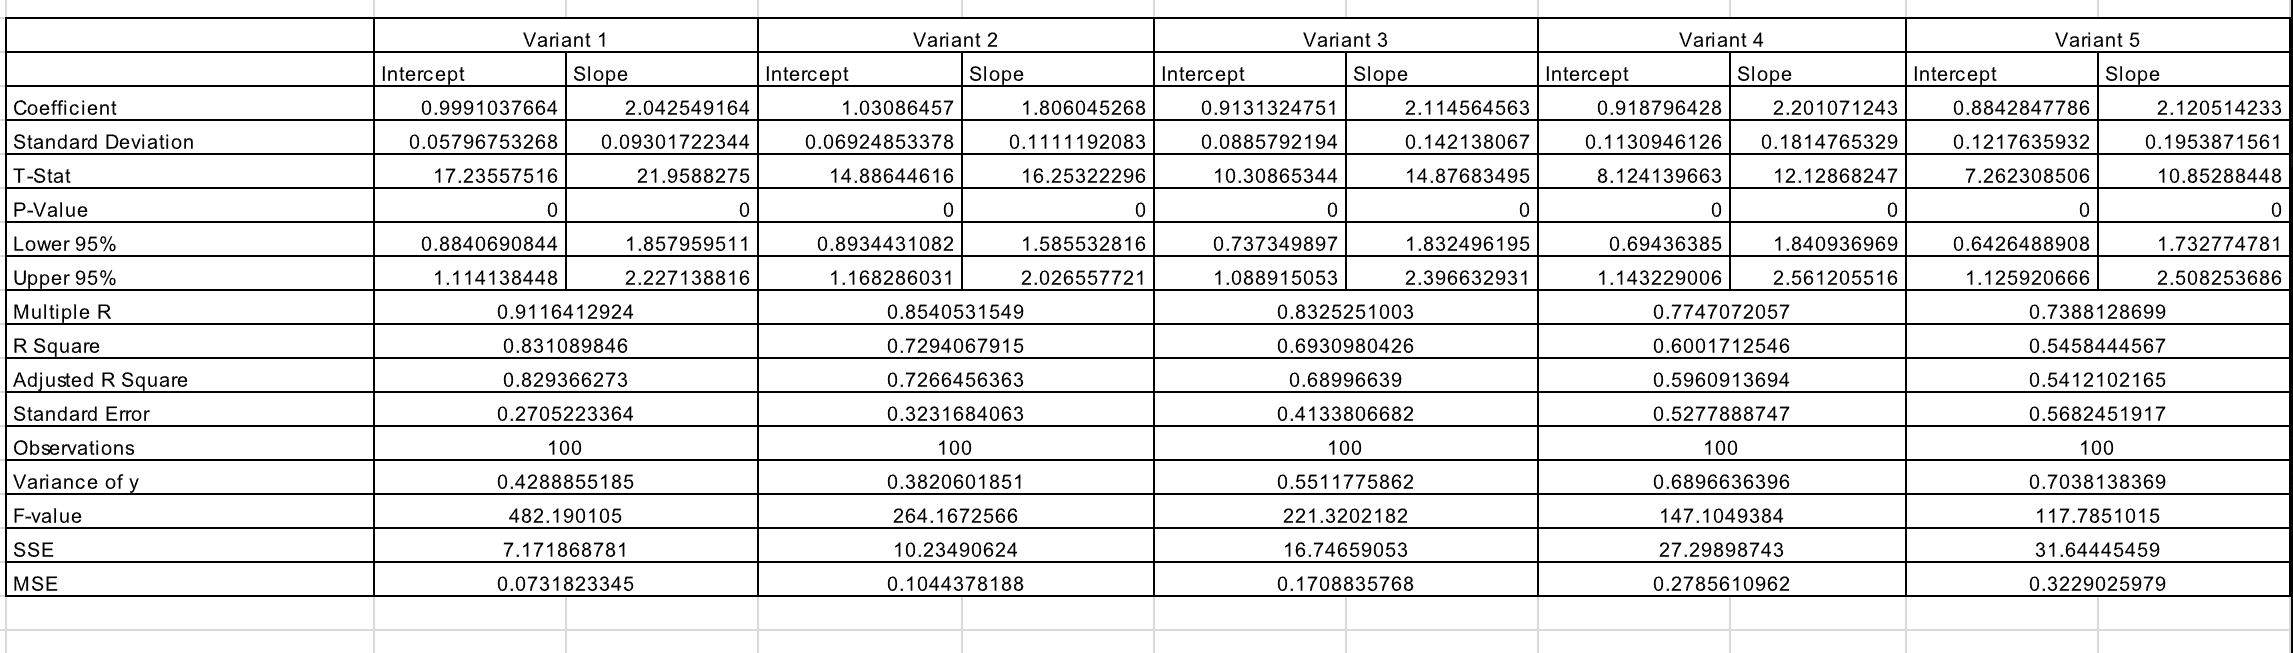
\includegraphics[width=\textwidth]{Images/Q4_1.png}
	\caption{Regression outcomes for each variant tabulated together}
	\label{fig:Q4.1}
\end{figure}

\vspace{10mm}

\begin{custombox}[label={box:Q4.2}]{Question 4.2}
	Create a plot of $R^2$ v/s variance (of $y$). What do you observe? Why?
\end{custombox}

The plot of $R^2$ v/s variance (of $y$) is shown in Figure \ref{fig:Q4.2}.

\begin{figure}[H]
	\centering
	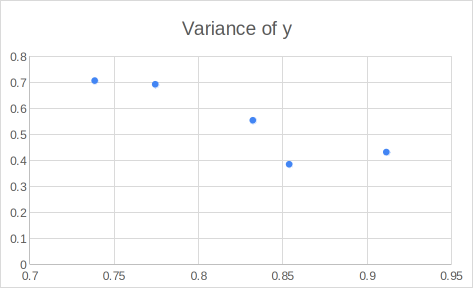
\includegraphics[width=0.5\textwidth]{Images/Q4_2.png}
	\caption{Plot of $R^2$ v/s variance (of $y$)}
	\label{fig:Q4.2}
\end{figure}

From the plot, we can observe that as the variance of $y$ increases, the value of $R^2$ decreases. This is because the variance of $y$ is a measure of how spread out the data is. When the variance of $y$ is high, the data is more spread out and the regression line fits the data less well. This results in a lower value of $R^2$.

\vspace{10mm}

\begin{custombox}[label={box:Q4.3}]{Question 4.3}
	Analyze the effect of variance on the regression parameters and prediction errors and state your observations and conclusions.
\end{custombox}

As the variance of $y$ increases, the regression parameters and prediction errors are affected as follows:

\begin{itemize}
	\item The value of $R^2$ decreases as the variance of $y$ increases. This indicates that the regression line fits the data less well when the data is more spread out.
	\item The $p$-value increase as the variance of $y$ increases. This indicates that the regression line is less statistically significant when the data is more spread out.
	\item The $F$-value decreases as the variance of $y$ increases. This indicates that the regression line is less significant when the data is more spread out.
	\item The sum of squared errors (SSE) and mean squared error (MSE) increase as the variance of $y$ increases. This indicates that the prediction errors are higher when the data is more spread out.
	\item The standard error values associated with the coefficients increase as the variance of $y$ increases. This indicates that the coefficient estimates are less accurate when the data is more spread out.
\end{itemize}

In conclusion, the variance of $y$ has a significant effect on the regression parameters and prediction errors. When the variance of $y$ is high, the regression line fits the data less well, the prediction errors are higher, and the coefficient estimates are less accurate.




